%Este trabalho está licenciado sob a Licença Atribuição-CompartilhaIgual 4.0 Internacional Creative Commons. Para visualizar uma cópia desta licença, visite http://creativecommons.org/licenses/by-sa/4.0/deed.pt_BR ou mande uma carta para Creative Commons, PO Box 1866, Mountain View, CA 94042, USA.

\chapter{Método de elementos finitos em 2D}\label{cap_mef2d}
\thispagestyle{fancy}

\section{Malha e espaço}\label{cap_mef2d_sec_malha}

\subsection{Malha}

Seja $\Omega\subset \mathbb{R}^2$ um domínio limitado com fronteira $\p\Omega$ suave e poligonal. Uma malha (ou triangularização) $\mathcal{K}$ de $\Omega$ é um conjunto de $\{K\}$ células (ou elementos) $K$, tal que $\Omega = \cup_{K\in\mathcal{K}}K$ e tal que a interseção de duas células é ou um lado, um canto ou vazio.

Classicamente as células $K$ são escolhidas como triângulos. O tamanho do lado de maior comprimento do triangulo $K$ define o chamado \emph{tamanho local da malha} $h_K$. O tamanho global da malha é definida por $h = \max_{K\in\mathcal{K}} h_K$.

Uma malha é dita \emph{regular} quando existe uma constante $c_0 > 0$ tal que $c_K > c_0$ para todo $K\in\mathcal{K}$, sendo $c_K := h_K/d_k$ e $d_K$ o diâmetro do circulo inscrito em $K$. Esta condição significa que os triângulo $K$ da malha não podem ter ângulos muito grandes nem muito pequenos. Ao longo do texto, a menos que especificado o contrário, assumiremos trabalhar com malhas regulares.

\subsection{Espaço dos polinômios lineares por partes}

Seja $K$ um triângulo e seja $P_1(K)$ o espaço das funções lineares em $K$, i.e.
\begin{equation}
  P_1(K) = \{v;~v=c_0+c_1x_1+c_2x+2,~(x_1,x_2)\in K,~c_0,c_1,c_2\in\mathbb{R}\}.
\end{equation}

Observemos que toda função $v\in P_1(K)$ é unicamente determinada por seus valores nodais $\alpha_i = v(N_i)$, $i=0, 1, 2$, onde $N_i = (x_1^{(i)}, x_2^{(i)})$ é o $i$-ésimo nodo (vértice) do triângulo $K$. Isto segue do fato de que
\begin{equation}
  \begin{bmatrix}
    1 & x_1^{(1)} & x_2^{(1)}\\
    1 & x_1^{(2)} & x_2^{(2)}\\
    1 & x_1^{(3)} & x_2^{(2)}
  \end{bmatrix}
  \begin{bmatrix}
    c_0\\
    c_1\\
    c_2
  \end{bmatrix} = 
  \begin{bmatrix}
    \alpha_1\\
    \alpha_2\\
    \alpha_3
  \end{bmatrix}
\end{equation}
Computando o valor absoluto do determinante da matriz de coeficientes, obtemos $2|K|$, onde $|K|$ denota a área de $K$, a qual é não nula.

Afim de usarmos os valores nodais como graus de liberdade (incógnitas), nós introduzimos a seguinte base nodal $\{\lambda_1, \lambda_2, \lambda_3\}$ com
\begin{equation}
  \lambda_j(N_i) = \left\{
    \begin{array}{ll}
      1 &, i=j,\\
      0 &, i\neq j
    \end{array}
\right.,~i,j=0,1,2.
\end{equation}
Com esta base, toda função $v\in P_1(K)$ pode ser escrita como
\begin{equation}
  v = \alpha_1\lambda_1 + \alpha_2\lambda_2 + \alpha_3\lambda_3,
\end{equation}
onde $\alpha_i = v(N_i)$.

\subsection{Espaço contínuo dos polinômios lineares por partes}

O espaço contínuo dos polinômios lineares por partes na malha $\mathcal{K}$ é definido por
\begin{equation}
  V_h = \{v;~v\in C^0(\Omega),~v|_K\in P_1(K),~\forall K\in\mathcal{K}\}.
\end{equation}

Observemos que toda função $v\in V_h$ é unicamente determinada por seus valores nodais $\{v(N_j)\}_{j=1}^{n_p}$, onde $n_p$ é número de nodos da malha $\mathcal{K}$. De fato, os valores nodais determinam uma única função em $P_1(K)$ para cada $K\in\mathcal{K}$ e, portanto, uma função em $V_h$ é unicamente determinada por seus valores nos nodos. Agora, consideremos dois triângulos $K_1$ e $K_2$ compartilhando um lado $E = K_1\cap K_2$. Sejam $v_1$ e $v_2$ os dois únicos polinômios em $v_1\in P_1(K_1)$ e $v_2\in P_2(K_2)$, respectivamente determinados pelos valores nodais em $K_1$ e $K_2$. Como $v_1$ e $v_2$ também são polinômios lineares em $E$ e seus valores coincidem nos nodos de $E$, temos $v_1 = v_2$. Portanto, concluímos que toda função $v\in V_h$ é unicamente determinada por seus valores nodais.

Afim de termos os valores nodais como graus de liberdade (incógnitas), definimos a base nodas $\{\phi_j\}_{j=1}^{n_p}\subset V_h$ tal que
\begin{equation}
  \varphi_j(N_i) = \left\{
    \begin{array}{ll}
      1 &, i=j\\
      0 &, i\neq j
    \end{array}
\right.,~i,j=0, 1, \dotsc, n_p-1.
\end{equation}
Notemos que cada função base $\phi_j$ é contínua, linear por partes e com suporte somente em um pequeno conjunto de triângulos que compartilham o nodo $N_j$. Além disso, todo a função $v\in V_h$ pode, então, ser escrita como
\begin{equation}
  v = \sum_{i=0}^{n_p-1}\alpha_i\varphi_i,
\end{equation}
onde $\alpha_i = v(N_i)$, $i=0, 1, \ldots, n_p$, são os valores nodais de $v$.

\begin{ex}\label{ex:malha}
  A Figura \ref{fig:ex_malha} mostra o esboço de uma malha triangular no domínio $D = [0, 1]\times [0, 1]$.

  \begin{figure}[h!]
    \centering
    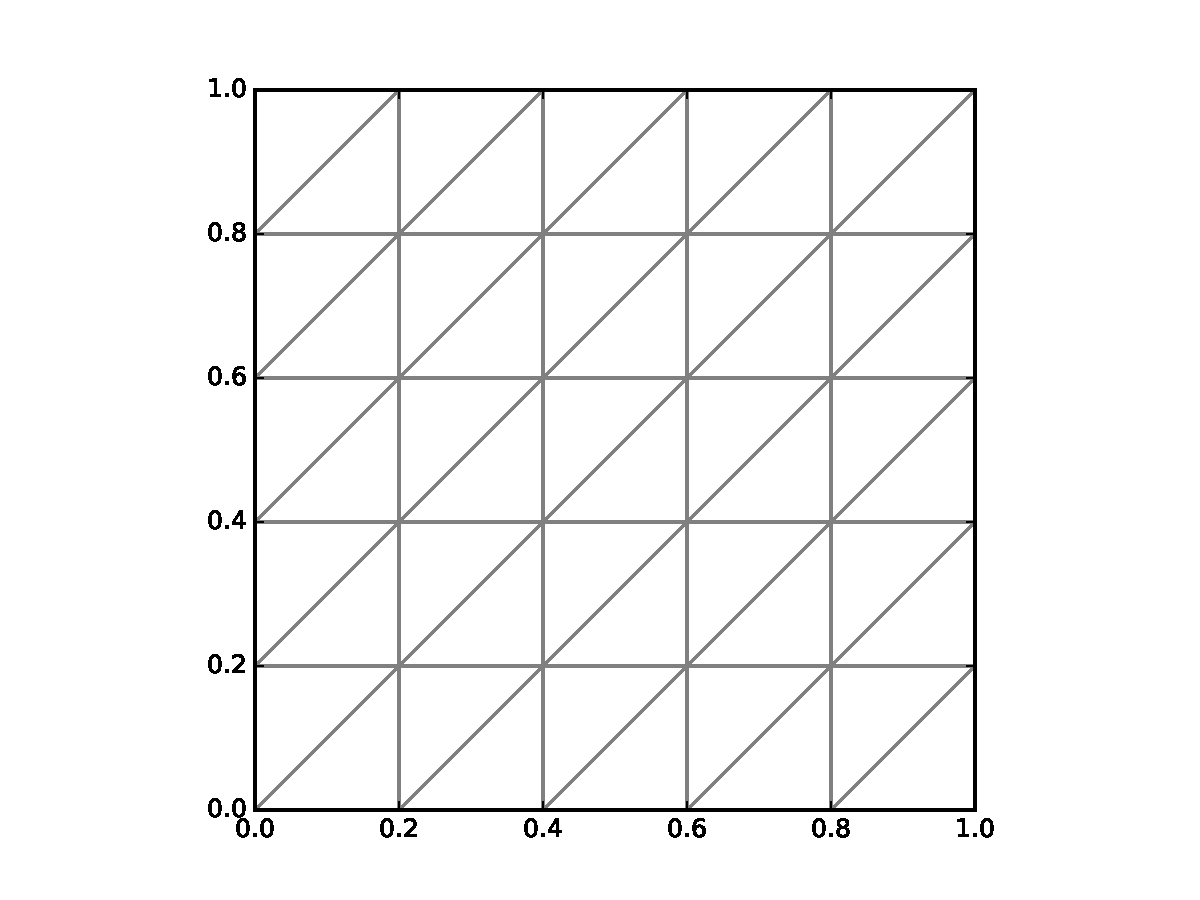
\includegraphics[width=0.7\textwidth]{./cap_mef2d/dados/ex_malha/fig_ex_malha}
    \caption{Esboço de uma malha triangular no domínio $D = [0, 1]\times [0, 1]$.}
    \label{fig:ex_malha}
  \end{figure}

\ifispython
Com o \fenics, podemos gerar esta malha com o seguinte \href{https://github.com/phkonzen/notas/blob/master/src/MetodoElementosFinitos/cap_mef2d/dados/ex_malha/ex_malha.py}{código}:
\verbatiminput{./cap_mef2d/dados/ex_malha/ex_malha.py}
\fi
\end{ex}

\section{Interpolação e projeção}\label{cap_mef2d_sec_interp}

\subsection{Interpolação}

Dada uma função contínua $f$ em um triângulo $K$ com nodos $N_i$, $i=0, 1, 2$, sua interpolação linear $\phi f \in P_1(K)$ é definida por
\begin{equation}
  \pi f = \sum_{i=0}^3 f(N_i)\varphi_i.
\end{equation}
Logo, temos $\pi f(N_i) = f(N_i)$ para todo $i=0, 1, 2$.

Afim de determinarmos estimativas para o erro de interpolação, precisamos da chamada derivada total de primeira ordem
\begin{equation}
  Df = \left(\left|\frac{\p f}{\p x_1}\right|^2 + \left|\frac{\p f}{\p x_2}\right|^2\right)^{1/2},
\end{equation}
e da derivada total de segunda ordem
\begin{equation}
  D^2f = \left(\left|\frac{\p^2 f}{\p x_1^2}\right|^2 + \left|\frac{\p^2 f}{\p x_1\p x_2}\right|^2 + \left|\frac{\p^2 f}{\p x_2^2}\right|^2\right)^{1/2}.
\end{equation}

\begin{prop}\normalfont{(Erro da interpolação no espaço linear)}\label{prop:interpl}
  A interpolação $\pi f$ satisfaz as seguintes estimativas
  \begin{align}
    \|f - \pi f\|_{L^2(K)} &\leq Ch_K^2\|D^2f\|_{L^2(K)},\label{eq:interpl_0}\\
    \|D(f - \pi f)\|_{L^2(K)} &\leq Ch_K\|D^2 f\|_{L^2(K)}.\label{eq:interpl_1}
  \end{align}
\end{prop}
\begin{dem}
  Veja \cite[Capítulo 4]{Brenner2008a}.
\end{dem}

\begin{obs}
  A constante $C$ dependo do inverso de $\sen(\theta_K)$ onde $\theta_K$ é o menor angulo de $K$. Desta forma, para um triângulo com $\theta_K$ muito pequeno, as estimativas \eqref{eq:interpl_0} e \eqref{eq:interpl_1} perdem sentido. Este fato indica a necessidade de se trabalhar com malhas regulares.
\end{obs}

A interpolação no espaço $V_h$ de uma dada função $f$ no domínio $\Omega$ é denotada também por $\pi f\in V_h$ e definida por
\begin{equation}
  \pi f = \sum_{i=0}^{n_p-1} f(N_i)\varphi_i.
\end{equation}

\begin{prop}\normalfont{(Erro da interpolação no espaço contínuo linear por partes)}\label{prop:interpc}
  O interpolador $\pi f\in V_h$ satisfaz as seguintes estimativas
  \begin{align}
    \|f - \pi f\|_{L^2(\Omega)}^2 &\leq C\sum_{K\in\mathcal{K}} h_K^4\|D^2 f\|_{L^2(K)}^2,\label{eq:interpc_0}\\
    \|D(f - \pi f)\|_{L^2(\Omega)}^2 &\leq C\sum_{K\in\mathcal{K}} h_K^2\|D^2 f\|_{L^2(K)}^2,\label{eq:interpc_1}.
  \end{align}
\end{prop}
\begin{dem}
  Demonstração análoga a Proposição \ref{prop:interp_linpartes}.
\end{dem}

\ifispython
\begin{ex}\label{ex:interp}
Consideremos a função $f(x_0,x_1) = \sen(\pi x_0)\cos(\pi x_1)$ definida no domínio $D = [0, 1]\times [0, 1]$. O seguinte \href{https://github.com/phkonzen/notas/blob/master/src/MetodoElementosFinitos/cap_mef2d/dados/ex_interp/ex_interp.py}{código} computa a interpolação de $f$ no espaço $V_h$ sobre uma malha triangular uniforme.

\verbatiminput{./cap_mef2d/dados/ex_interp/ex_interp.py}
\end{ex}
\fi

\subsection{Projeção $L^2$}

A projeto $L^2$ no espaço $V_h$ de uma dada uma função $f\in L^2(\Omega)$  é denotada por $P_hf\in V_h$ e definida por
\begin{equation}
  \int_\Omega (f-P_hf)v\,dx = 0,~\forall v\in V_h.
\end{equation}

Analogamente a projeção em uma dimensão (veja Subseção \ref{subsec:projecao_1d}), a projeção
\begin{equation}
  P_h f = \sum_{j=0}^{n_p-1} \xi_j\varphi_j,
\end{equation}
onde $\xi_j$ satisfaz o sistema linear
\begin{equation}
  M\pmb{\xi} = \pmb{b},
\end{equation}
onde $M = [m_{i,j}]_{i,j=0}^{n_p-1}$ é a matriz de massa com
\begin{equation}
  m_{i,j} = \int_{\Omega} \varphi_i\varphi_j\,dx
\end{equation}
e $\pmb{b} = (b_1,~b_2,~\dotsc,~b_{n_p-1})$ é o vetor de carga com
\begin{equation}
  b_i = \int_\Omega f\varphi_i\,dx.
\end{equation}

Também, vale o resultado análogo da melhor aproximação (veja \ref{teo:melhor_aprox}), i.e.
\begin{equation}
  \|f-P_hf\|_{L^2(\Omega)} \leq \|f - v\|_{L^2(\Omega)},\quad\forall v\in V_h.
\end{equation}
E, portanto, também temos a estimativa análoga para o erro de projeção (veja \ref{teo:erro_proj_1d})
\begin{equation}
  \|f-P_hf\|_{L^2(\Omega)}^2 \leq C\sum_{K\in\mathcal{K}} h_K^4\|D^2 f\|_{L^2(K)}^2.
\end{equation}
Tomando o tamanho global da malha, temos
\begin{equation}\label{eq:erro_projec_2d}
  \|f-P_hf\|_{L^2(\Omega)} \leq Ch^2\|D^2 f\|_{L^2(K)}.
\end{equation}

\ifispython
\begin{ex}\label{ex:projec}
Consideremos a função $f(x_0,x_1) = \sen(\pi x_0)\cos(\pi x_1)$ definida no domínio $D = [0, 1]\times [0, 1]$. O seguinte \href{https://github.com/phkonzen/notas/blob/master/src/MetodoElementosFinitos/cap_mef2d/dados/ex_projec/ex_projec.py}{código} computa a projeção de $f$ no espaço $V_h$ sobre uma malha triangular uniforme.

\verbatiminput{./cap_mef2d/dados/ex_projec/ex_projec.py}
\end{ex}
\fi

\subsection*{Exercícios}

\begin{exer}
  Verifique computacionalmente a Proposição \ref{prop:interpc} no caso da função $f(x_0,x_1) = \sen(\pi x_0)\cos(\pi x_1)$ interpolada sobre uma malha triangular uniforme sobre o domínio $D = [0, 1]\times [0, 1]$.
\end{exer}

\begin{exer}
  Verifique computacionalmente a estimativa \eqref{eq:erro_projec_2d} no caso da função $f(x_0,x_1) = \sen(\pi x_0)\cos(\pi x_1)$ projetada sobre uma malha triangular uniforme sobre o domínio $D = [0, 1]\times [0, 1]$.
\end{exer}

\section{Problema modelo}\label{cap_mef2d_sec_probmodelo}

Nesta seção, apresentaremos a aplicação do método de elementos finitos para a equação de Poisson\footnote{Siméon Denis Poisson, 1781 - 1840, matemático francês. Fonte: \href{https://en.wikipedia.org/wiki/Sim\%C3\%A9on_Denis_Poisson}{Wikipedia}.} com condições de Dirichlet\footnote{Johann Peter Gustav Lejeune Dirichlet, 1805 - 1859, matemático alemão. Fonte: \href{https://en.wikipedia.org/wiki/Peter_Gustav_Lejeune_Dirichlet}{Wikipedia}.}, i.e.: encontrar $u$ tal que
\begin{align}
  -\Delta u &= f,~x\in\Omega,\label{eq:mef2d_pm_eq}\\
  u &= 0,~x\in\p\Omega,\label{eq:mef2d_pm_bc}
\end{align}
onde $\Delta = \p^2/\p x_0^2 + \p^2/\p x_1^2$ é o operador de Laplace\footnote{Pierre-Simon, marquis de Laplace, 1749 - 1827, matemático francês. Fonte: \href{https://en.wikipedia.org/wiki/Pierre-Simon_Laplace}{Wikipedia}.} e $f$ é uma função dada.

\subsection{Formulação variacional}

A aplicação do método de elementos finitos é construída sobre a formulação fraca do problema \eqref{eq:mef2d_pm_eq}-\eqref{eq:mef2d_pm_bc}. Para obtermos esta, multiplicamos \eqref{eq:mef2d_pm_eq} por uma função teste $v$ em um espaço adequado $V_0$ e integramos no domínio $\Omega$, i.e.
\begin{equation}
  - \int_\Omega \Delta uv\,dx = \int_\Omega fv\,dx.
\end{equation}
Então, usando a fórmula de Green\footnote{George Green, 1793 - 1841, matemático britânico. Fonte: \href{https://en.wikipedia.org/wiki/George_Green_(mathematician)}{Wikipedia}.}, obtemos
\begin{equation}
  \int_\Omega \nabla u\cdot\nabla v\,dx - \int_\Omega n\cdot\nabla uv\,ds.
\end{equation}
Então, observando critérios de regularidade e a condição de contorno \eqref{eq:mef2d_pm_bc}, escolhemos
\begin{equation}
  V_0 := \{v\in H^1(\Omega):~v|_{\p\Omega}=0\}.
\end{equation}
Lembramos que $H^1(\Omega) = \{v:~\|v\|_{L^2(\Omega)}+\|\nabla v\|_{L^2(\Omega)}<\infty\}$.

Com isso, temos o seguinte problema fraco associado a \eqref{eq:mef2d_pm_eq}-\eqref{eq:mef2d_pm_bc}: encontrar $u\in V_0$ tal que
\begin{equation}\label{eq:mef2d_probfraco}
  a(u,v) = L(v),~\forall v\in V_0,
\end{equation}
onde $a(u, v)$ é chamada de forma bilinear e definida por
\begin{equation}
  a(u,v) := \int_\Omega \nabla u\cdot\nabla v\,dx
\end{equation}
e $L(v)$ é chamada de forma linear e definida por
\begin{equation}
  L(v) := \int_\Omega fv\,dx.
\end{equation}

\subsection{Formulação de elementos finitos}

A formulação de elementos finitos é obtida da formulação fraca \eqref{eq:mef2d_probfraco} pela aproximação do espaço teste $V_0$ por uma espaço de dimensão finita. Tomando uma triangulação $\mathcal{K}\subset\Omega$ e considerando o espaço contínuo dos polinômios lineares por partes
\begin{equation}
  V_h := \{v:~v\in C^0(\Omega), v|_K\in P_1(K)~\forall K\in\mathcal{K}\},
\end{equation}
assumimos também o subconjunto $V_{h,0}:= \{v\in V_h:~v|_{\p\Omega}=0\}$.

Com isso, temos o seguinte problema de elementos finitos associado \eqref{eq:mef2d_probfraco}: encontrar $u_h\in V_{h,0}$ tal que
\begin{equation}\label{eq:mef2d_probfem}
  a(u_h,v_h) = L(v_h),~\forall v_h\in V_{h,0}.
\end{equation}

Observemos que \eqref{eq:mef2d_probfem} é equivalente ao problema de encontrar $u_h\in V_{h,0}$ tal que
\begin{equation}\label{eq:mef2d_proba1}
  a(u_h,\varphi_i) = L(\varphi_i),
\end{equation}
com $i=0, 1, \cdots, n_p-1$, onde $\{\varphi_i\}_{i=0}^{n_i-1}$ é a base nodal de $V_{h,0}$ e $n_i$ é o número de funções bases (igual ao número de nodos internos da triangulação $\mathcal{K}$). Ainda, como
\begin{equation}
  u_h = \sum_{j=0}^{n_i-1} \xi_j\varphi_j,
\end{equation}
temos 
\begin{align}
  a(u_h, \varphi_i) &= a\left(\sum_{j=0}^{n_i-1}\xi_j\varphi_j,\varphi_i\right) \\
  &= \sum_{j=0}^{n_i-1}\xi_ja(\varphi_j,\varphi_i).
\end{align}

Com isso, o problema de elementos finitos é equivalente a resolver o seguinte sistema linear
\begin{equation}
  \sum_{j=0}^{n_i-1}\xi_ja(\varphi_j,\varphi_i) = L(\varphi_i),~i=0, 1, \cdots, n_i-1,
\end{equation}
para as incógnitas $\xi_j$, $j=0, 1, \cdots, n_i-1$. Ou, equivalentemente, temos sua forma matricial
\begin{equation}
  A\pmb{\xi} = \pmb{b},
\end{equation}
onde $A = [a_{i,j}]_{i,j=0}^{n_i-1}$ é chamada de \pmb{matriz de rigidez}\index{matriz de rigidez} com
\begin{equation}
  a_{i,j} = a(\varphi_j, \varphi_i)
\end{equation}
e $\pmb{b} = (b_0, b_1, \cdots, b_{n_i-1})$ é o vetor de carga com
\begin{equation}
  b_i = L(\varphi_i).
\end{equation}

\begin{ex}\label{ex:mef2d_pm}
  Consideremos o seguinte problema de Poisson
  \begin{align}
    -\Delta u &= x_0(1-x_0)x_1(1-x_1),~x\in\Omega:=(0, 1)\times (0, 1),\\
    u &= 0,~x\in\p\Omega.
  \end{align}
  Na Figura \ref{fig:mef2d_pm} temos um esboço da aproximação de elementos finitos obtida em uma malha uniforme com $20\times 20$ nodos. As isolinhas correspondem aos ponto tais que $u=3\times 10^{-1}, 2\times 10^{-1}$, $10^{-1}$, $5\times 10^{-2}$.

  \begin{figure}[h!]
    \centering
    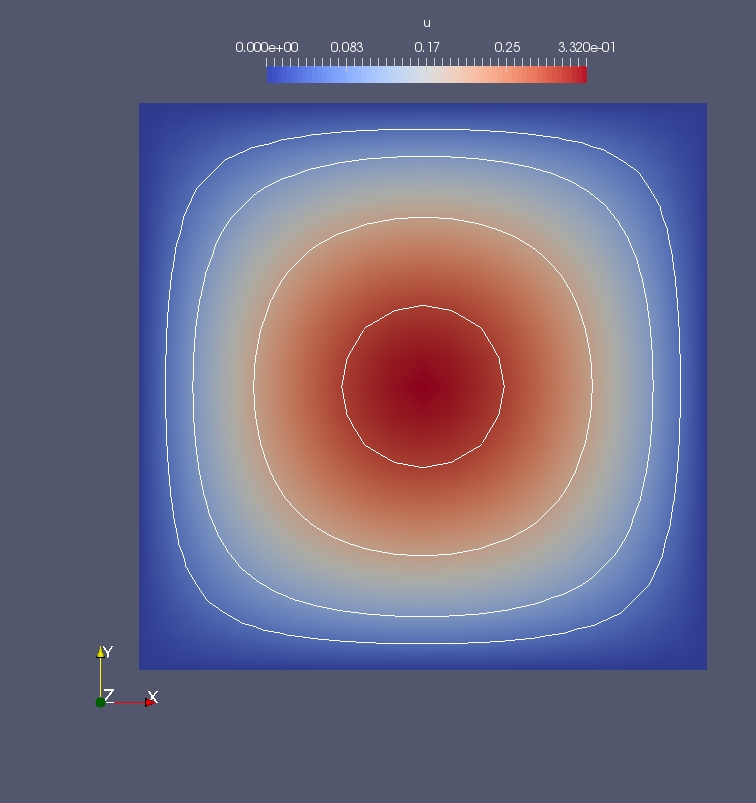
\includegraphics[width=0.7\textwidth]{./cap_mef2d/dados/ex_mef2d_pm/fig_mef2d_pm}
    \caption{Esboço da solução de elementos finitos do problema discutido no Exemplo \ref{ex:mef2d_pm}.}
    \label{fig:mef2d_pm}
  \end{figure}

\ifispython
Com o \fenics, podemos computar a solução deste problema com o seguinte \href{https://github.com/phkonzen/notas/blob/master/src/MetodoElementosFinitos/cap_mef2d/dados/ex_mef2d_pm/ex_mef2d_pm.py}{código}:
\verbatiminput{./cap_mef2d/dados/ex_mef2d_pm/ex_mef2d_pm.py}
\fi
\end{ex}

\subsection*{Exercícios}

\begin{exer}
  Compute uma aproximação de elementos finitos para o seguinte problema
\begin{align}
  -\Delta u &= 10,~x\in (0, 1)\times (0, 1)\\
  u(x,0) &= 0,~0\leq x \leq 1,\\
  u(1,y) &= 0,~0\leq y < 1,\\
  u(x,1) &= 1,~0\leq x \leq 1,\\
  u(0,y) &= 1,~0<x\leq 1.
\end{align}
\end{exer}

\section{Fundamentos da análise de elementos finitos}

\subsection{Existência e unicidade}

\begin{teo}\normalfont{(Matriz positiva definida)}\label{teo:matriz_definida_positiva}
  A matriz de rigidez é positiva definida.
\end{teo}
\begin{dem}
  A matriz de rigidez $A = [a(\varphi_j,\varphi_i)]_{ij=0}^{n_i-1}$ é obviamente simétrica. Além disso, para todo $\pmb{\xi}\in\mathbb{R}^{n_i}$, $\pmb{\xi}\neq 0$, temos
  \begin{align}
    \pmb{\xi}^TA\pmb{\xi} &= \sum_{i,j=0}^{n_i-1} \xi_ja(\varphi_j,\varphi_i)\xi_i\\
    &= \sum_{i,j=0}^{n_i-1}\xi_j\int_\Omega \nabla \varphi_j\cdot\nabla\varphi_i\,dx\\
    &= \int_\Omega \nabla \left(\sum_{j=0}^{n_i-1}\xi_j\varphi_j\right)\cdot\nabla \left(\sum_{i=0}^{n_i-1}\xi_i\varphi_i\right)\,dx\\
    &= \left\|\nabla \left(\sum_{j=0}^{n_i-1}\xi_j\varphi_j\right) \right\|_{L^2(\Omega)}^2.
  \end{align}
  Portanto, $\pmb{\xi}^TA\pmb{\xi} \leq 0$ e é nulo se, e somente se, $v = \sum_{j=0}^{n_i-1}\xi_j\varphi_j$ for constante. Como $v\in V_{h,0}$, temos que $v$ constante implica $v\equiv 0$, mas então $\pmb{\xi}=0$, o que é uma contradição. Logo, $\pmb{\xi}^TA\pmb{\xi} > 0$ para todo $\pmb{\xi}\in\mathbb{R}^{n_i}$, $\pmb{\xi}\neq 0$.
\end{dem}

\begin{teo}\normalfont{(Existência e unicidade)}
  O problema de elementos finitos \eqref{eq:mef2d_probfem} tem solução única.
\end{teo}
\begin{dem}
  O problema de elementos finitos \eqref{eq:mef2d_probfem} se resume a resolver o sistema linear $A\pmb{\xi} = \pmb{b}$. Do Teorema \ref{teo:matriz_definida_positiva}, temos que $A$ é uma matriz definida positiva e, portanto, invertível. Daí segue, imediatamente, que o problema \eqref{eq:mef2d_probfem} tem solução única.
\end{dem}

\subsection{Estimativa {\it a priori} do erro}

\begin{teo}\normalfont{(Ortogonalidade de Galerkin)}\label{teo:mef2d_orto_Galergin}
  A solução $u_h$ do problema de elementos finitos \eqref{eq:mef2d_probfem} satisfaz
  \begin{equation}
    a(u-u_h,v_h) = L(v_h),~\forall v_h\in V_{h,0},
  \end{equation}
onde $u$ é a solução do problema fraco \eqref{eq:mef2d_probfraco}.
\end{teo}
\begin{dem}
  Segue, imediatamente, do fato de que $V_{h,0}\subset V_0$ e, portanto,
  \begin{equation}
    a(u,v_h) = L(v_h),~\forall v_h\in V_{h,0},
  \end{equation}
bem como
  \begin{equation}
    a(u_h,v_h) = L(v_h),~\forall v_h\in V_{h,0}.
  \end{equation}
\end{dem}

\begin{defn}\normalfont{(Norma da energia.)}
  Definimos a norma da energia por
  \begin{equation}
    \||v|\| := \left(\int_{\Omega} \nabla v\cdot\nabla v\,dx\right)^{1/2} = \|\nabla v\|_{L^2(\Omega)},
  \end{equation}
para todo $v\in V_0$.
\end{defn}

\begin{teo}\normalfont{(Melhor aproximação.)}\label{teo:mef2d_melhor_aprox}
  A solução $u_h$ do problema de elementos finitos satisfaz
  \begin{equation}
    \||u-u_h|\| \leq \||u-v_h|\|,~\forall v_h\in V_{h,0}.
  \end{equation}
\end{teo}
\begin{dem}
  Observando que $u-u_h=u-v_h+v_h-u_h$ e usando a ortogonalidade de Galerkin (Teorema \ref{teo:mef2d_orto_Galerkin}), temos:
  \begin{align}
    \||u-u_h|\|^2 &= \int_\Omega \nabla (u-u_h)\cdot\nabla (u-u_h)\,dx\\
    &= \int_{\Omega} \nabla (u-u_h)\cdot\nabla (u-v_h)\,dx + \int_{\Omega} \nabla (u-u_h)\cdot\nabla (v_h-u_h)\,dx\\
    &= \int_{\Omega} \nabla (u-u_h)\cdot\nabla (u-v_h)\,dx\\
    &= \|\nabla (u-u_h)\|_{L^2(\Omega)}^2\|\nabla (u-v_h)\|_{L^2(\Omega)}^2\\
    &= \||u-u_h|\|^2\||u-v_h|\|.
  \end{align}
\end{dem}

\begin{teo}\normalfont{(Estimativa {\it a priori} do erro.)}\label{teo:mef2d_est_apriori_energia}
  A solução $u_h$ do problema de elementos finitos \eqref{eq:mef2d_probfem} satisfaz
  \begin{equation}
    \||u-u_h|\|^2 \leq C\sum_{K\in\mathcal{K}} h_K^2\|D^2u\|_{L^2(K)}^2.
  \end{equation}
\end{teo}
\begin{dem}
  O resultado segue do Teorema da melhor aproximação (Teorema \ref{teo:mef2d_melhor_aprox}) e da estimativa do erro de interpolação (Proposição \ref{prop:interpc}), pois
  \begin{align}
    \||u-u_h|\|^2 \leq \||u-\pi u|\|^2\\
    = \|D(u-\pi u)\|_{L^2(\Omega)}^2\\
    \leq C\sum_{K\in\mathcal{K}} h_K^2\|D^2u\|_{L^2(\Omega)}^2.
  \end{align}
\end{dem}

Para obtermos uma estimativa na norma $L^2(\Omega)$, podemos usar a desigualdade de Poincaré.

\begin{teo}\normalfont{(Desigualdade de Poincaré.)}
  Seja $\Omega\subset \mathbb{R}^2$ um domínio limitado. Então, existe uma constante $C = C(\Omega)$, tal que
  \begin{equation}
    \|v\|_{L^2(\Omega)} \leq C\|\nabla v\|_{L^2(\Omega)},~\forall v\in V_0.
  \end{equation}
\end{teo}
\begin{dem}
  Se $\Omega$ tem contorno suficientemente suave, então existe $\phi$ tal que $-\Delta \phi = 1$ em $\Omega$ com $\sup_{x\in\Omega}|\nabla \phi| < C$. Com isso, temos
  \begin{align}
    \|v\|_{L^2(\Omega)}^2 &= \int_{\Omega} v^2\,dx\\
    &= -\int_{\Omega} v^2\Delta\phi\,dx.
  \end{align}
Agora, usando o Teorema de Green e a desigualdade de Cauchy-Schwarz, obtemos
\begin{align}
  \|v\|_{L^2(\Omega)}^2 &= -\int_{\p\Omega} v^2n\cdot\nabla \phi\,ds + \int_\Omega \nabla v^2\cdot\nabla \phi\,dx\\
  &= \int_\Omega 2v\nabla v\cdot\nabla \phi\,dx\\
  &\leq \sup_{x\in\Omega} |\nabla \phi|\|v\|_{L^2(\Omega)}\|\nabla v\|_{L^2(\Omega)}.
\end{align}
\end{dem}

Com a desigualdade de Poincaré e da estimativa {\it a priori} do erro (Teorema \ref{teo:mef2d_est_apriori_energia}), temos
\begin{equation}\label{eq:mef2d_est_apriori}
  \|u-u_h\|_{L^2(\Omega)} \leq C \||u-u_h|\| \leq Ch\|D^2u\|_{L^2(\Omega)},
\end{equation}
onde $h = \max_{K\in\mathcal{K}} h_K$. Entretanto, esta estimativa pode ser melhorada.

\begin{teo}\normalfont{(Estimativa ótima {\it a priori} do erro.)}
  A solução $u_h$ do problema de elementos finitos \eqref{eq:mef2d_probfem} satisfaz
  \begin{equation}
    \|u-u_h\|_{L^2(\Omega)} \leq Ch^2\|D^2u\|_{L^2(\Omega)}.
  \end{equation}
\end{teo}
\begin{dem}
  Seja $e = u-u_h$ o erro e $\phi$ a solução do problema dual (ou problema adjunto)
  \begin{align}
    -\Delta \phi &= e,~\forall x\in\Omega\\
    \phi &= 0,~\forall x\in\p\Omega.
  \end{align}
Então, usando a fórmula de Green, a ortogonalidade de Galerkin e, então, a desigualdade de Cauchy-Schwarz, temos
\begin{align}
  \|e^2\|_{L^2(\Omega)} &= -\int_\Omega e\Delta\phi\,dx\\
  &=\int_\Omega \nabla e\cdot\nabla\phi\,dx - \int_{\p\Omega} en\cdot\nabla \phi\,ds\\
  &=\int_\Omega \nabla e\cdot\nabla(\phi-\pi\phi)\,dx\\
  \leq\|\nabla e\|_{L^2(\Omega)}\|\nabla(\phi-\pi\phi)\|_{L^2(\Omega)}.
\end{align}
Da estimativa {\it a priori} \eqref{eq:mef2d_est_apriori} (que segue do Teorema \ref{teo:mef2d_est_apriori_energia}) temos
\begin{equation}
  \|\nabla e\|_{L^2(\Omega)} \leq Ch\|D^2u\|_{L^2(\Omega)}.
\end{equation}
Agora, da regularidade elíptica $\|D^2\phi\|_{L^2(\Omega)} \leq C\|\Delta\phi\|_{L^2(\Omega)}$ \cite{Evans1998a} e da estimativa do erro de interpolação (Proposição \ref{prop:interpc}), temos
\begin{equation}
  \|\nabla(\phi-\pi\phi)\|_{L^2(\Omega)} \leq Ch\|D^2\phi\|_{L^2(\Omega)}\leq Ch\|\Delta\phi\|_{L^2(\Omega)} \leq Ch\|e\|_{L^2(\Omega)}.
\end{equation}
Então, temos
\begin{equation}
  \|e\|_{L^2(\Omega)}^2 \leq Ch\|D^2u\|_{L^2(\Omega)}Ch\|e\|_{L^2(\Omega)}.
\end{equation}
\end{dem}
